\chapter{Усадьба Светославского}

Идя вдоль Кирилловских высот на северо-запад к Смородинскому спуску, к Логову Змиеву, нельзя обойти вниманием бывшую усадьбу Светославского – она обозначена на карте Хвойки буквой «Е» и находилась на отроге, следующем по счету после большого мыса принадлежащего Зарембскому, а позже Бернеру. 

С большой долей вероятности предположу место бывшей усадьбы Светославского на аэрофотоснимке 1943 года там, где видим прогрызенный глинищами (я отнес их к заводу Бернера) холм, северо-западный «укус». Адрес на 1911 год – Кирилловская, 77. Координаты примерно 50°28'39.2"N 30°29'01.4"E. В 2014 году это закрытый северо-западный въезд на Богуславский спуск, через дорогу от зеленого трехэтажного дома по Кирилловской 96. Семье Светославских в начале 20 века принадлежали и усадьбы на четной стороне улицы, по Кирилловской 94-96, но зеленый дом – не их, а кажется построен позже. Всё это считалось Куренёвкой.

Из книги в книгу, из уст в уста, маститые ученые, экскурсоводы и краеведы повторяют, что Куренёвка называлась так от казачьих куреней, мол, на окраине селились казаки, которым не давали жить в пределах Подола. Но в этих краях и выше по Сырцу стояли винокурни. Есть даже приток Сырца – Курячий брод. В 18 веке на Сырце было 29 винокурень, а на Приорке и Куренёвке из 84 усадеб-хуторов на 64-х работали винокурни. Тут курили – «гнали» спиртное. Слово «выкурить» вообще употреблялось к вину, дегтю, смоле. И по обилию винокурень – Куреневка.

В двухтомнике «История Киева» 1963 года усадьба Светославского отнесена к несуществующему ныне адресу Кирилловская, 81. Как бы ни было, между Богуславским и Смородинском спуском (ближе к первому), по обе стороны Кирилловской улицы, владела земельными участками семья Светославских, в их числе художник-пейзажист Светославский Сергей Иванович (1857-1931). Что видел, то и рисовал – благодаря чему у нас остались замечательные живописные полотна окрестностей Кирилловской улицы.

\begin{center}
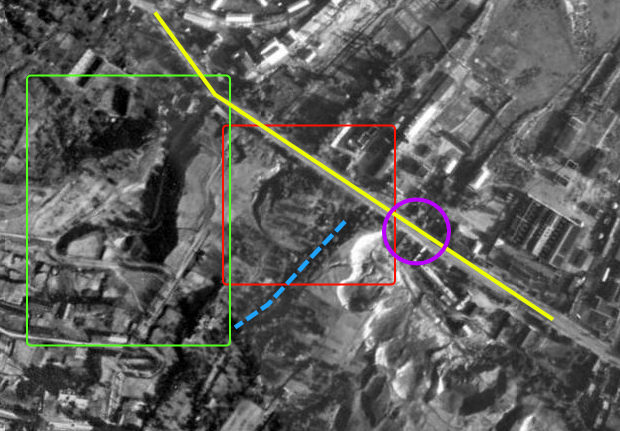
\includegraphics[width=\linewidth]{chast-kirvys/svetosl/sveto-aero.jpg}
\end{center}

На аэрофотоснимке 1943 года я отметил примерное место верхней усадьбы Светославских – посередине красного прямоугольника. Желтая линия – улица Кирилловс\-кая. Фиолетовый круг – нынешний перекресток Кирилловской и Нахимова. Самая левая точка этого круга – теперь северо-восточный конец Богуславского спуска. Зеленый прямоугольник – Смородинский спуск. Голубой пунктир – ручей в овраге. Этот овраг пробуривает гору к переулку Нагорному. Другой овраг как бы огибает часть склона восточнее.

Представим, что сейчас 2014 год. Отмеченная красным область относительно не застроена, пребывает в одичавшем виде, поэтому совершим по ней короткую прогулку. Миновав, по Кирилловской, закрытый воротами выход из Богуславского спуска, сразу свернем налево, там будет бровка небольшой подпорной стены. Между нею и холмом, параллельно улице идет тропка. Вдоль тропы над землей проложены две трубы, а под землей в коллекторе течет, отведенный перпендикулярно основному руслу в овраге, ручей. Скоро доходим до этого оврага и становимся к нему лицом.

\begin{center}
\includegraphics[width=\linewidth]{chast-kirvys/svetosl/\myimgprefix IMG_3659.JPG}

\textit{В овраге. 2014 год.}
\end{center}

Можно двинуться по оврагу прямо, либо свернуть направо, мимо деревянного столба электропередачи – таких по пути встретится несколько – лестничкой, переходящей в мощеную мелким булыжником дорожку. Рано или поздно, покружив около суглинного мыса, она выведет к Нагорному переулку. Слева и справа от дорожки – заросшие бурьяном площадки, вероятно места бывших строений. У первого поворота, если пойти дальше сквозь чащу – остатки некоего подземного сооружения. Они выглядят как бетонная, без крыши, коробка. Слева от нее земля провалилась в пустоту, кажется, что коробка заняла б\'ольшую ее объема полость. 

Если подниматься по усеянному битым кирпичом оврагом, чьи берега почти отвесны, а по обеим сторонам торчат развалины, мы доберемся до места, где ручей спускается в коллектор. К нему он подведен по бетонному желобу. Еще юго-западнее желоба ручей бежит в естественном русле через бурелом и мусор, среди которого я нашел ржавую, но сохранившую цвета, красно-сине-белую табличку «Застрахован в Варшавском обществе» – такие страховые таблички висели на домах до революции. 

Вдоль ручья можно двигаться до поры до времени, ибо наступает момент, когда ноги увязают в размоченной почве. Поднимемся на левый склон оврага и осторожно, дабы не сорваться, пойдем по кромке между обрывом и кривым деревянным забором. Через дыры в заборе зеленеют заросли диких задворков Татарки, откуда, за пустырем, через противоположную дыру есть выход на другую сторону отрога. Приближаемся к началу оврага. Ограниченный с трех сторон крутыми склонами, ручей вытекает внизу из трубы в западном.

Таковы окрестности бывшей усадьбы Светославских. Ни дом его, ни другие строения тут не сохранились. Всё заросло деревьями, кустами, крапивой, и странно, что сюда способны проникать люди и стаскивать мусор.

Сергей Светославский родился в Киеве, в 1857 году, в семье мелкого чиновника Ивана Светославского, из дворян, благодаря чему после революции художник был лишен права голосования. В 1862-м Светославские переехали – Псков, Питер, Тверская губерния. В 1875 году Сергей Иванович поступил в Московское училище живописи, скульптуры и архитектуры. Преподавали ему Саврасов – пейзаж, Перов – рисование человека, Поленов. Вместе со Светославским учились братья Коровины, Левитан. Сергей Иванович временно перешел из училища в Петербургскую Академию искусств, потом вернулся в Москву, в 1883 году летом путешествовал по Руси – писал этюды – и опоздал к началу занятий в училище, за что был исключен. Но диплом учителя рисования всё равно получил, да еще серебряную медаль. В 1884 году потянуло снова в Киев, к родителям на Куреневку, Кирилловскую улицу. 

Выставки, медали. Писал картину за картиной –  большая часть наследия художника хранится теперь в Национальном художественном музее Украины. Примкнул к рядам передвижников. Дружил с Васнецовым, Пимоненко, Шишкиным, Поленовым, Маковским, Левитаном, Константином Коровиным, Серовым. Васнецов написал со Светославского голову Моисея на фронтоне Владимирского собора.

Васнецов во время работы над оформлением храма, с 1885 года, жил в Киеве. Прибыл сюда с женой и двухлетним сыном. В статье А. В. Васнецова об отце – «Воспоминания о Викторе Михайловиче Васнецове» – я нашел про Светославского:

\begin{quotation}
Ближе всего мы были с семьей проф Прахова. Кроме них ходили к нам художники: Ковалевский, Менк, Сведомский, Котарбинский, Светославский, который жил на горе под Киевом. Как-то мы ездили к нему на «гору Светославского», как говорили. Помню, долго надо было подыматься вверх, где стоял дом, помню большую темноватую мастерскую, павлиньи перья на камине, а больше ничего не помню.
\end{quotation}

Это важное свидетельство. Обычно полагают, что Светославский всё время жил на четной, низинной стороне улицы, в то время как эти слова Васнецова убеждают в обратном – художник какие-то годы обитал именно на горе, ее склоне.

Однако вот нижняя усадьба, дореволюционное полотно, слева – Кирилловские высоты, за забором одноименная улица, вид на северо-запад.

\begin{center}
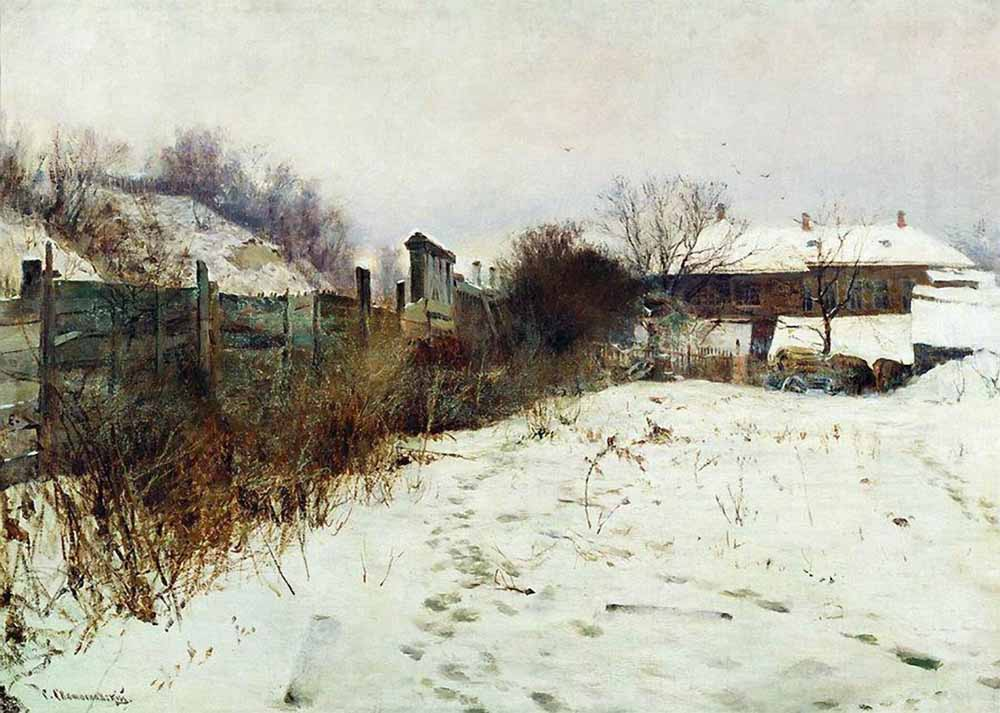
\includegraphics[width=0.95\linewidth]{chast-kirvys/svetosl/sveto-usadba-hudojnika-zimoy.jpg}

\textit{Светославский. «Усадьба художника зимой».}
\end{center}

И нижняя усадьба в 1931 году, вид на северо-восток из оврага в склоне Кирилловских высот, через улицу: 

\begin{center}
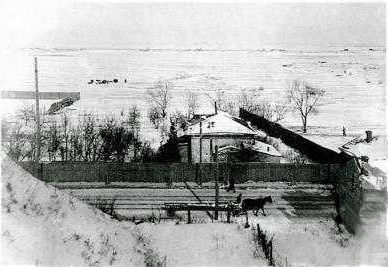
\includegraphics[width=0.95\linewidth]{chast-kirvys/svetosl/1931.jpg}
\end{center}

\begin{center}
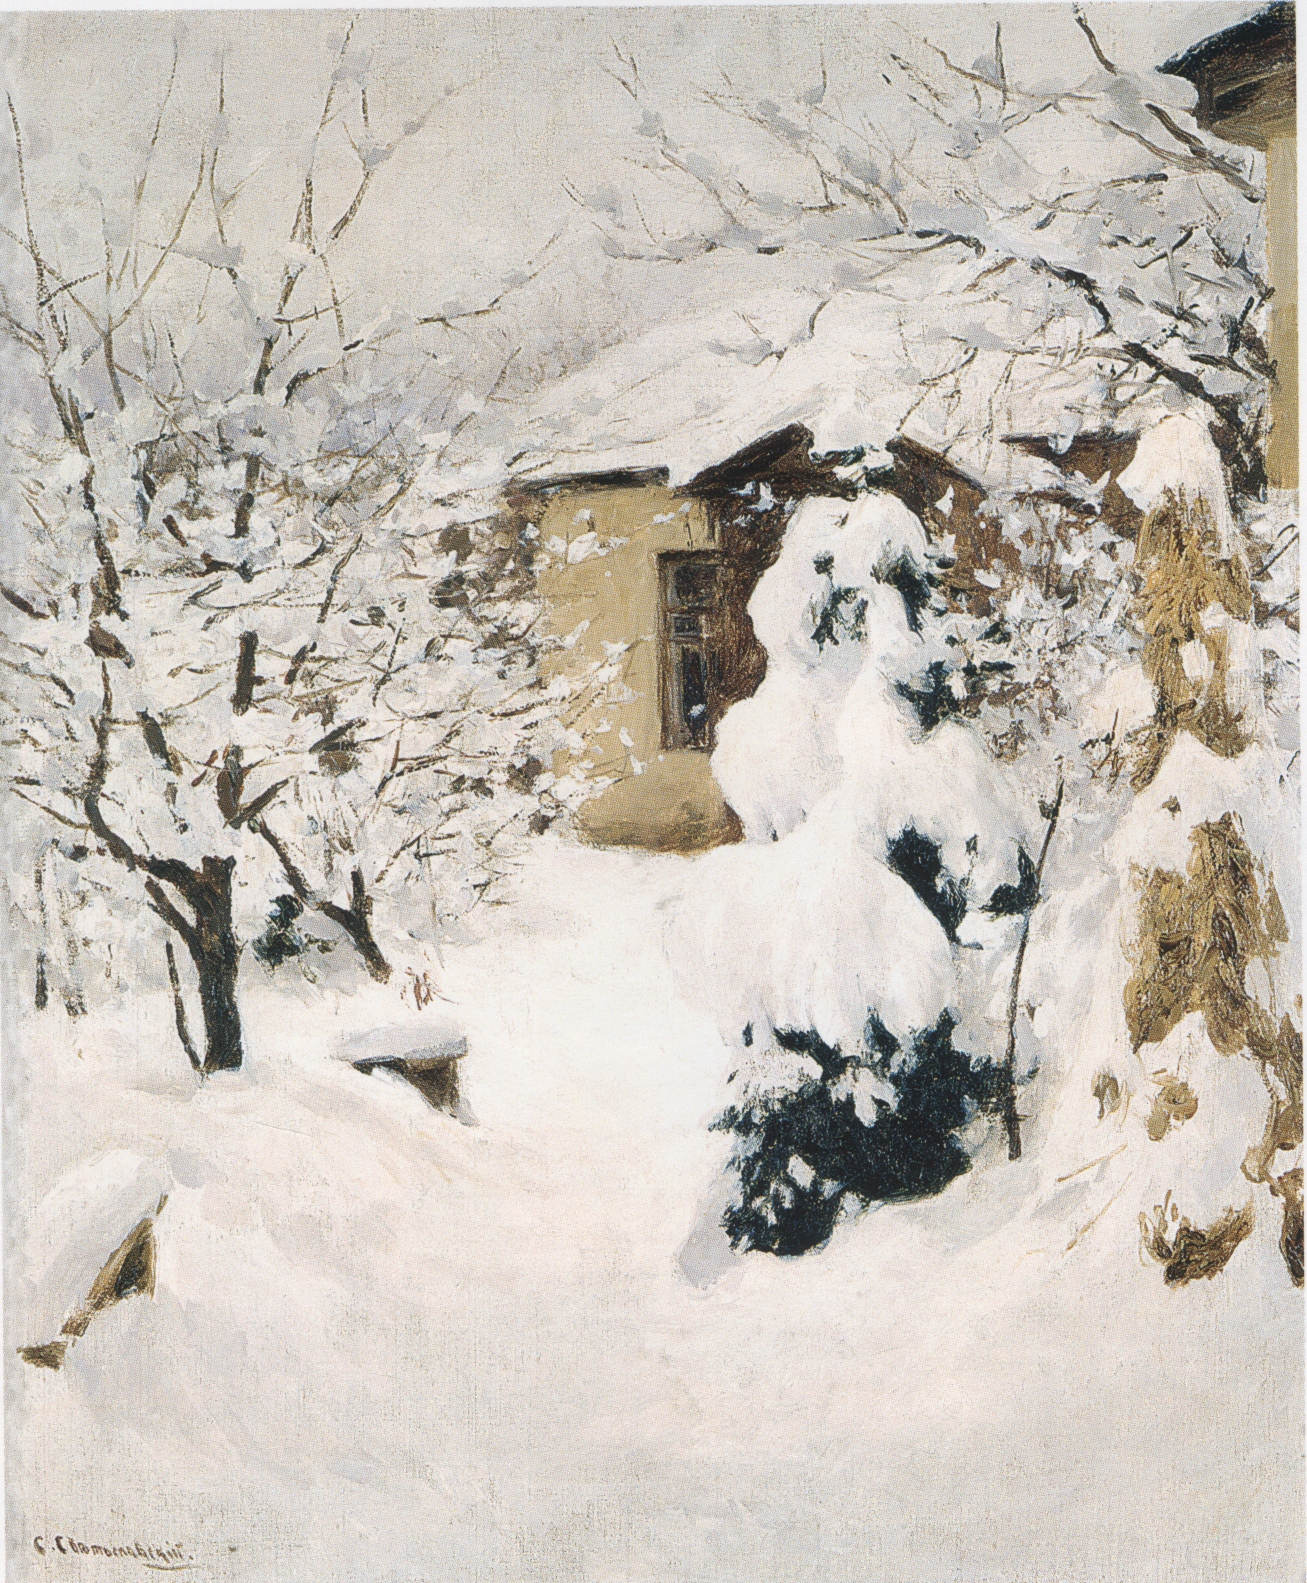
\includegraphics[width=\linewidth]{chast-kirvys/svetosl/sveto-zimniy-peizaj-usadba-hud-19xx.jpg}

\textit{Светославский, начало 20 века. Зимний пейзаж. Усадьба художника.}
\end{center}

В 1890 году Сергей Иванович женился на Александре Петровне Юргенсон, поселился с нею в Москве, на Покровке, в Колпашном переулке. Через четыре года развелся. Опять в Киев. Путешествия, выставки. Вышел из Товарищества передвижников. Стал почетным членом в Киевском отделе Товарищества любителей животных, доставляя животных в новосозданный в 1908 году зоопарк. Выбивал под него деньги, например у известного Третьякова. 

В 1910 году Светославский продал часть усадьбы на Кирилловской улице и за вырученные деньги отправился в Среднюю Азию, за новыми зверями. Это была не первая его подобная экспедиция. А в 1917 году, когда животные зоопарка голодали и Светославский через газету обратился открытым письмом за помощью к депутатам Киевской городской думы, то помещенных за решетку зверей он именует «узниками». Переосмысление их судьбы?

В половодье на Оболони и Подоле, Сергей Иванович на своей лодке плавал и спасал людей, помогал обездоленным материально.

Картины художник зачастую отдавал на благотворительные выставки – некоторые устраивались и обществом защиты животных. Жертвовал деньги Красному кресту. В 1905 создал бесплатную студию, поначалу для сорока студентов Киевского художественного училища, которых оттуда вытурили за участие в забастовках.

Среди учеников новой студии, просуществовавшей несколько лет, были Александр Архипенко, Александр Богомазов (жил на Вознесенском спуске), Алексей Грищенко, София Левицкая. Первые два ушли потом в авангард. Светославский советовал студентам: «Наблюдайте весну. Идите в парки. Наблюдайте одно и то же место ежедневно и ежечасно, и вы увидите, как изменяется природа».

К тому времени, и нижней усадьбе, относятся воспоминания товарища Светославского, М. Ковалевского, чья жена училась живописи:

\begin{quotation}
Усадьбу от улицы отделял длинный некрашеный забор […] За забором был небольшой участок земли, который почти весь во время разлива Днепра заливала вода. На незатопляемой части усадьбы стояли два небольших деревянных домика. В одном жила старенькая мать художника, а в другом, переоборудованном под мастерскую, жил он сам. Его семейная жизнь сложилась неудачно. В молодости он бракосочетался с москвичкой Юргенсон, но очень скоро они разошлись, и с того времени Светославский жил с матерью и братом, которых очень нежно и преданно любил.
\end{quotation}

Тогда Светославский был полон сил и выглядел «крепким, подтянутым мужчиной среднего возраста, лысым, с длинной курчавой бородой и с бронзовым загорелым лицом – недавно вернулся из Средней Азии. На первый взгляд он походил на пожилого узбека: этому очень способствовала и тюбетейка, которую он тогда носил».

\vspace*{\fill}


\begin{center}
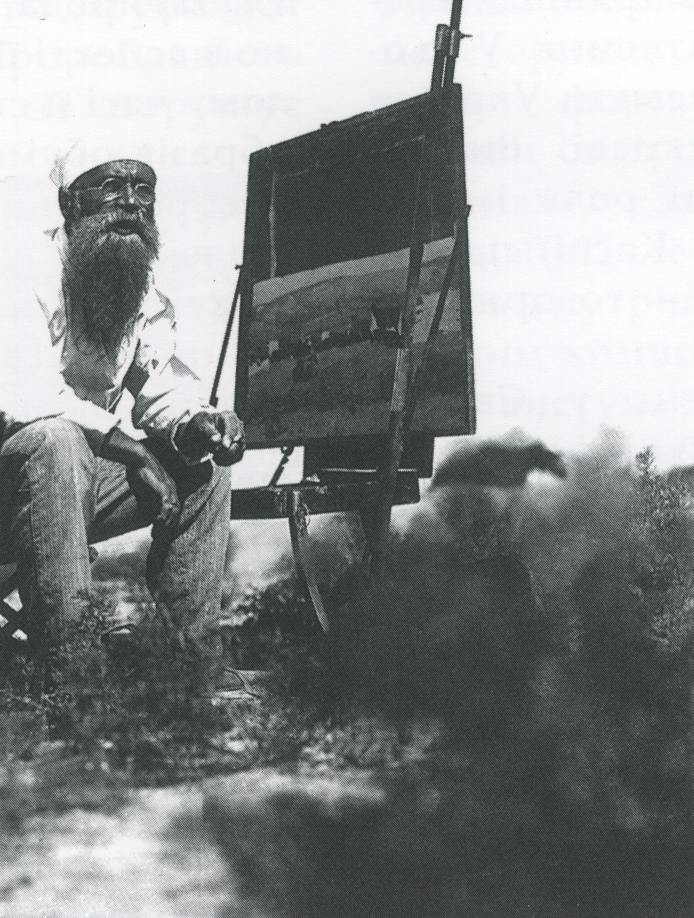
\includegraphics[width=0.80\linewidth]{chast-kirvys/svetosl/sveto-port.jpg}

\textit{Светославский за работой. Фотография начала 20 века.}
\end{center}

\newpage

Потом всё закрутилось. Первая мировая, революция, гражданка – чехарда ужаса, ставшего нормой. А Светославский теряет зрение. Мир уменьшился до усадьбы под Кирилловскими высотами, которую он доселе много рисовал. Устанавливается новая власть, ей художник не нужен, забыто его заступничество за революционных студентов, устройство зоопарка. А Светославский не видит – не может завершить большое полотно в половину мастерской. Сколько этюдов остались только зародышами будущих картин!

В неспокойное время гибнущую усадьбу под горой посещали мрачные люди и предлагали – жизнь или золото. Светославский отвечал, что его золото – в глазах и пальцах. Мрачные искали другое золото. Рылись среди недописанных картин. Ничего. Уходили.

А приспособился. Красил за деньги заборы, продавал на базаре выращенную на огороде картошку да петрушку. Мастерил для продажи ведра, сковородки.

Художник Федор Зотикович Коновалюк, бывший ученик Светославского, знавший его до революции, отправился проведать своего учителя. С гостинцем. Калитку отворил сам хозяин усадьбы, заросший, больной. Коновалюк будто не узнал его и спросил: «Здесь ли живет художник Светославский?». На что получил ответ: «Художник Светославский давно умер». 

19 сентября 1931 года Сергей Иванович Светославский умер и был похоронен на Лукьяновском кладбище.

Как случилось, что художника, которого ставили вровень с Левитаном, а работы покупали Третьяков и Терещенко, постепенно забыли? Усадьбу, где можно было сделать музей, снесли, картины лежат в разных запасниках да частных коллекциях.

%Несколько статей в сети, россыпь воспоминаний в разных источниках, публичное забвение – никакой улицы имени, никакого музея, разве что впервые за многие десятилетия, в 2003 году провели выставку «Свет Сергея Светославского». И снова – в небытие.

Следуя тому же, что советовал ученикам, Светославский рисовал порой одно и то же место в разные времена года. 1890-е, две картины – «Окраина Киева. Зима» и «Окраина Киева. Лето. Куреневка» доносят нам вид и настроение Кирилловских высот того времени. Громоздятся один над другим домики, лестнички, перила, сады, сараи.

И третье полотно конца 19 века, «Окраина Киева». Снова видим кручу Кирилловских высот, проулок с косым забором и домиком, какие стояли еще, кажется полвека и женщину в розовой рубахе будто с фотографии Прокудина-Горского. Женщина набирает воду в ведра, а вода бежит по системе деревянных желобов, проведенных от склона, переливаясь из одного в другой. Не удивлюсь, если подобные «трубы» применялись и возле Иорданской церкви для подачи воды из верхнего источника в нижний колодец.
\vspace*{\fill}
\begin{center}
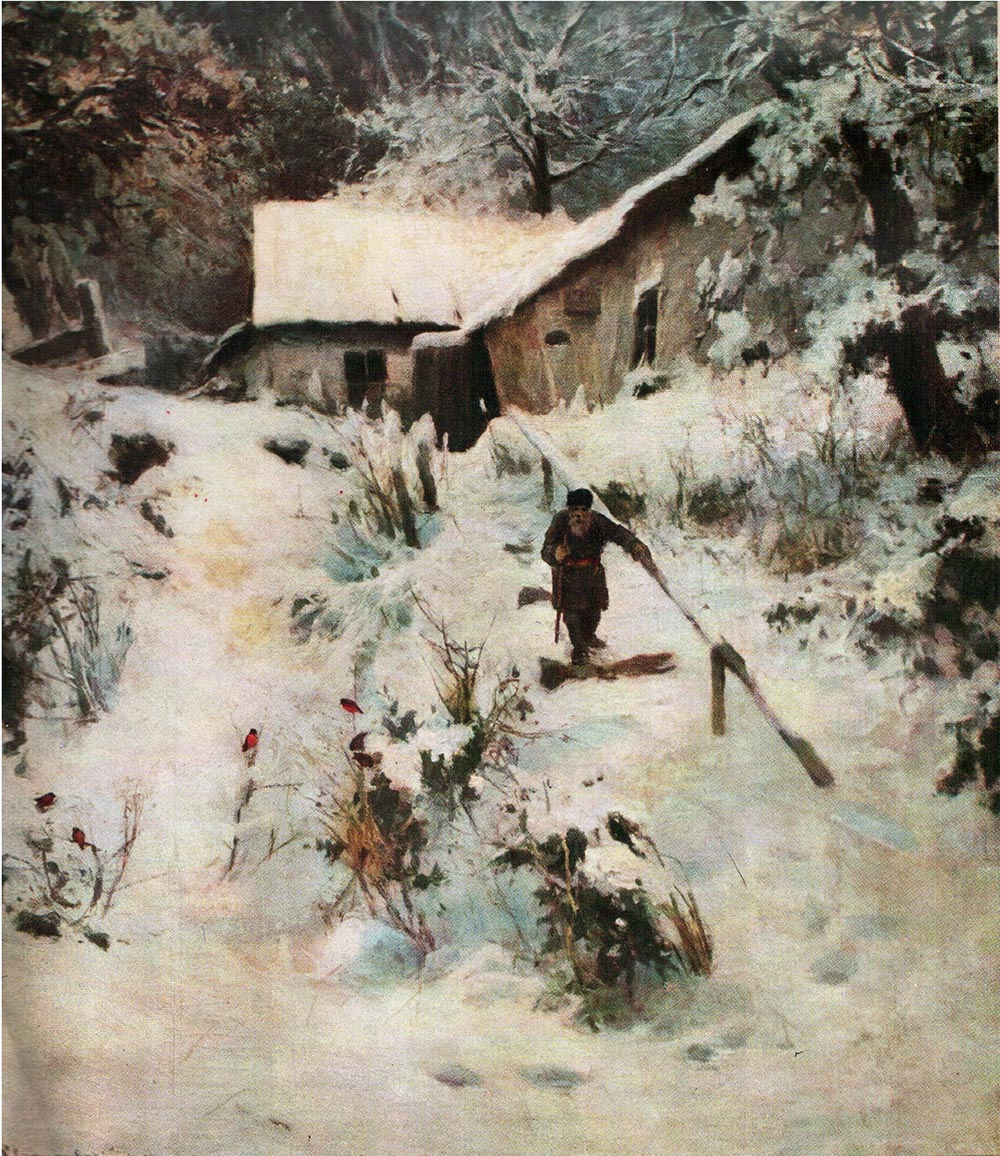
\includegraphics[width=\linewidth]{chast-kirvys/svetosl/sveto-1890-okraina-kieva-zima.jpg}

\textit{Светославский. Окраина Киева. Зима.}
\end{center}
\vspace*{\fill}
\newpage

\vspace*{\fill}
\begin{center}
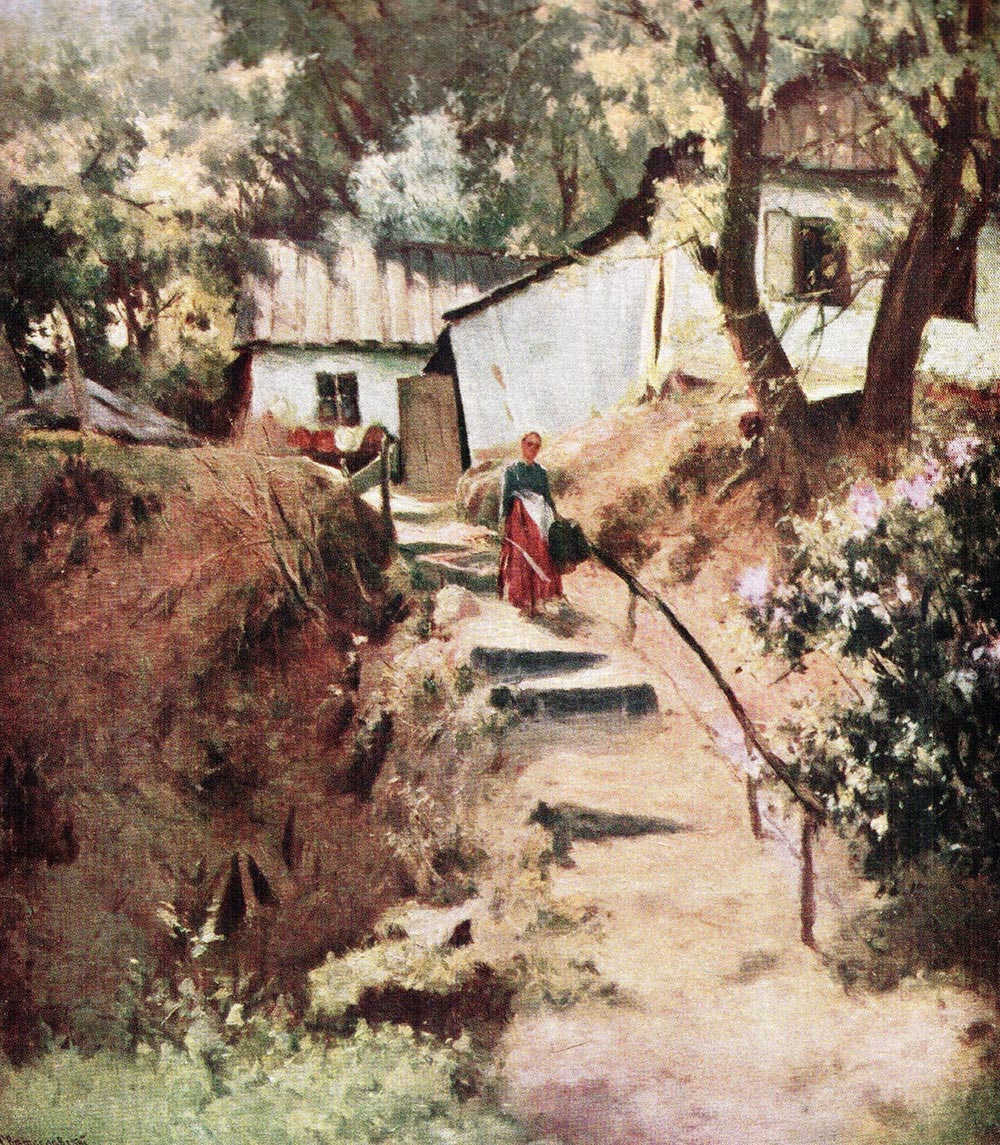
\includegraphics[width=\linewidth]{chast-kirvys/svetosl/sveto-1890-okraina-kieva-leto-kurenevka.jpg}

\textit{Светославский. Окраина Киева. Лето. Куреневка.}
\end{center}

\vspace*{\fill}

\newpage

«Окраина Киева»:

\begin{center}
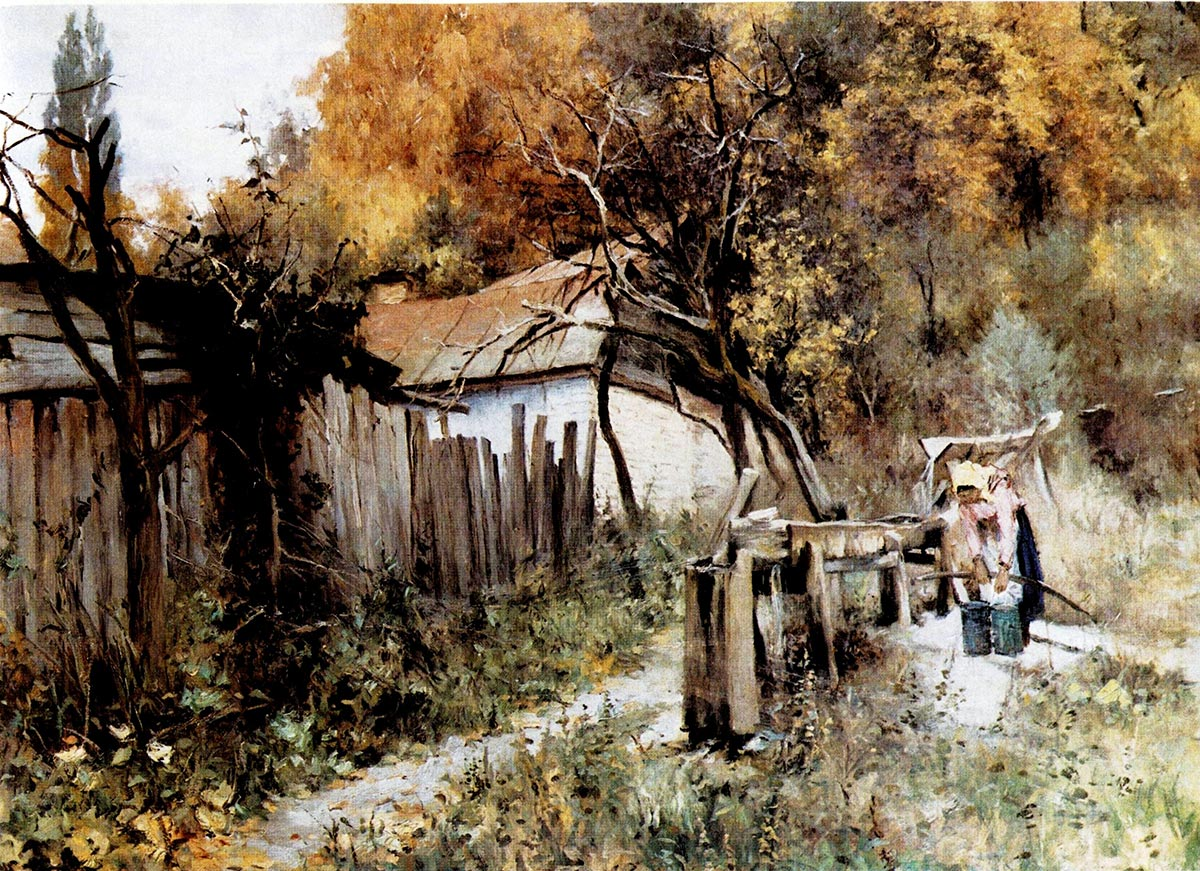
\includegraphics[width=\linewidth]{chast-kirvys/svetosl/sveto-1890-okraina-kieva.jpg}
\end{center}

А эта картина называется «Разлив»:

\begin{center}
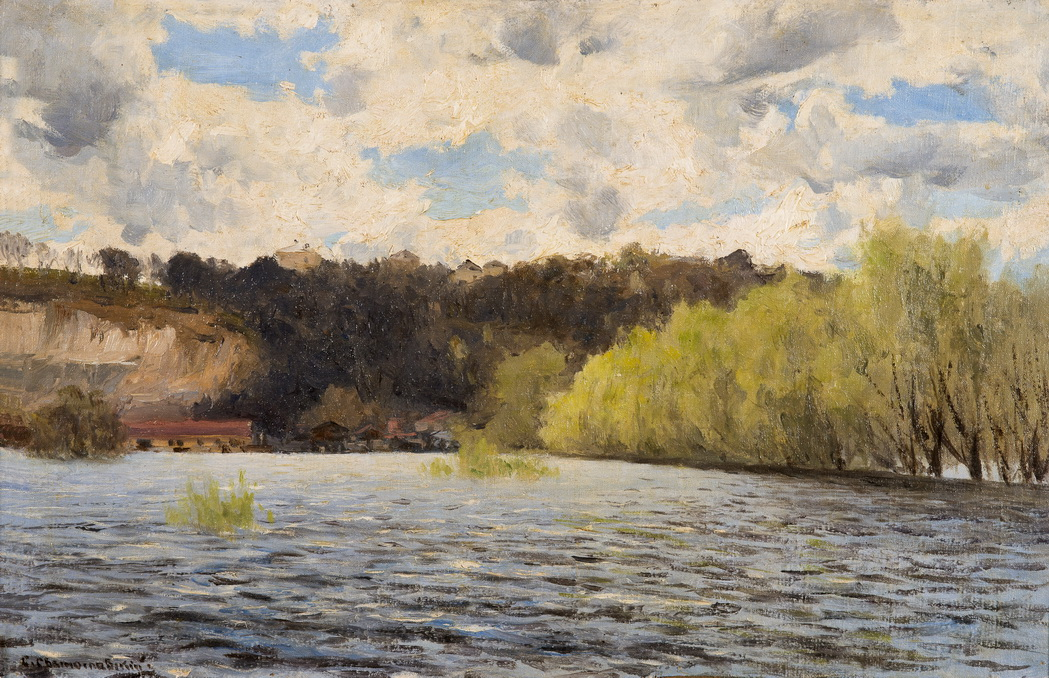
\includegraphics[width=\linewidth]{chast-kirvys/svetosl/sveto-razliv.jpg}
\end{center}

Здесь Кирилловские высоты во всей шири. Вода дошла к самым домикам на Кирилловской улице, внизу. Слева – обвалившийся, или, скорее, разрытый кирпичным заводом склон. Наверху – здания уже Лукьяновки или Татарки, тогда не различали.

Вот что пишет Викентий Хвойка в своей монументальной статье «Каменный век среднего Приднепровья»:

\begin{quotation}
Осенью 1895 года мне пришлось сопровождать профессора Феофилактова, пожелавшего исследовать расположение слоев Киевских возвышенностей, примыкающих к Кирилловской улице. С этой целью мы зашли, между прочим, в усадьбу г. Светославского, где в это время производилась съемка горы\footnote{То есть срывали склон.} и, следовательно, представлялась возможность для наблюдения профессором интересовавших его слоев.

Узнавший о цели нашего прихода владелец усадьбы сообщил нам, что у него на горе часто находят разные куски глиняных черепков и что между ними его сторож нашел однажды какого-то глиняного идольчика.

Заинтересованные этим сообщением, мы последователи за любезным хозяином в его мастерскую, где мое любопытство было еще более возбуждено при виде показанных нам образцов сделанных находок, состоявших из черепков и частей сосудов, во многих случаях позволявших угадывать их первоначальную форму. Черепки эти по своей выделке, составу материала и совершенно новому для нашей местности типу представляли нечто до такой степени своеобразное и не похожее на сделанные мною раньше находки, что я немедленно обратился к г. Светославскому с просьбой разрешить мне раскопать некоторые места в его усадьбе, на что без затруднения получил самое любезное согласие.

Не теряя времени, я на другой же день, взяв с собой одного из моих рабочих, приступил к раскопкам, начав с месте, показанного на плане под №1\footnote{План смотрите далее.}.

Место это находится на самом плато возвышенности, которая, сливаясь в одну общую нагорную поверхность, тянется довольно крутым скатом до самой Кирилловской улицы, возвышаясь над ней в роде отдельного мыса.

Избранное нами место составляло часть одной стенок прорезанной через него дороги, при прокладке которой и были обнаружены находящиеся в земле глиняные черепки; 
\end{quotation}

Хвойка приводит следующий план местности (в лучшем качестве у меня нет), где цифрами археолог обозначил места раскопов.

\begin{center}
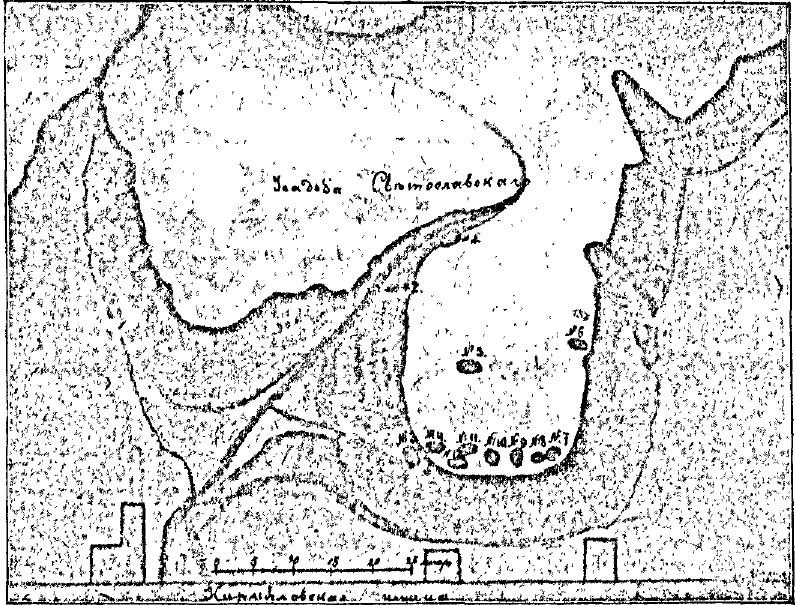
\includegraphics[width=\linewidth]{chast-kirvys/svetosl/sveto.png}
\end{center}
 
Хвойка продолжает:

\begin{quotation}
здесь же была найдена весьма интересная статуэтка из темно-красной глины, представляющая собой женскую фигуру, лицо которой имело вид треугольника, а крючковатый нос и большие, близко поставленные глаза придавали все физиономии сходство с собой (табл. XX, №5)
\end{quotation}

В скане, который мне доступен, таблица XX отсутствует, поэтому картинку разместить не могу. Хвойка дальше пишет, что продолжая там рыть, на глубине 35 сантиметров стал находить черепки. Еще через 55 сантиметров он откопал большой очаг, дном уходящий в лёсс. В очаге была зола, черепки разбитых сосудов, угли, речные ракушки Unio pictorum и Anodonta cygnaea, причем, как рассказывает Хвойка:

\begin{quotation}
Большая часть найденных черепков отличалась чрезвычайно изящной выделкой; независимо от тонкости и нежности глины, по выделке и составу приближающейся к греческой терракоте, поверхность их была очень искусно приглажена и расписана темно-коричневыми разводами
\end{quotation}

\begin{center}
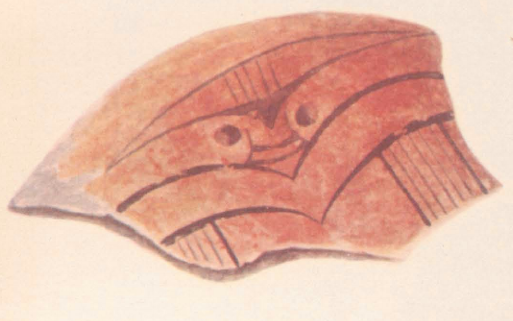
\includegraphics[width=0.70\linewidth]{chast-kirvys/svetosl/svet-keramika.png}
\end{center}

\begin{quotation}
Несмотря на все это, найденные черепки не внушали никого сомнения в том, что они были сделаны без помощи гончарного круга, прямо от руки. Из числа этих черепков нас более всего поразила часть сосуда, наполненного невскрытыми ракушками; поверхность его была покрыта по оранжево-желтому фону темно-коричневым орнаментом из волнообразных линий и треугольников. Из числа других черепков и частей разбитых сосудов в особенности выдавались или украшенные разного вида ушками и выпуклостями, или имеющие донышко на трех и более ножках, или же те, края которых были косо срезаны, а также имеющие настолько сглаженную поверхность, что они казались как будто покрытыми лаком.

Кроме черепков, между ракушками, комками обожженной глины, разбитыми костями животных, птиц и рыб мы нашли два довольно больших и прекрасно отделанных кремневых ножа и несколько кремневых предметов, а также несколько камней со следами обработки и часть фигурки из черной глины, изображающую человеческую голову с обозначением на ней  глаз и сильно загнутого носа, без всяких признаков рта.

В золе кострища мы нашли несколько шишкообразных лепешек, подобных найденным в предыдущих раскопках, и, как и те, служивших вероятно пищей жившего здесь человека.

Измерить все занятое описанное предметами пространство нам не удалось, так как почти половина исследуемого нами места была уничтожена при проведении чрез него дороги, для которой потребовалась съемка земли более чем на 2 1/2 м., но уцелевшая его часть в самом широком месте (считая и уступ вокруг ямы с очагом, где было найдено много предметов) имела около 4 м.
\end{quotation}

Хвойка продолжил копать в окрестностях. Ему попадались другие очаги, закопченные остатки печей для приготовления пищи, полуземлянки в лёссе, черепки, глиняные прясла, щиты пресноводной черепахи, обломки кремневых ножей, кремневые наконечники стрел, некие предметы хорошей отделки «из костей птиц, рыб и четвероногих животных; лучшими представителями последних могут служить предметы из клыков кабана». Всё это лежало в «смеси ракушек, костей животных и птиц и костей и чешуи рыбы» – стало быть, в бытовом мусоре.

В раскопе номер 4, который оказался уже разрыт генералом Багговутом, Хвойка отыскал, помимо черепков и кремневых орудий, «небольшое полукруглое сооружение из выжженной докрасна глины, поверхность которого была окрашена белой краской и, несмотря на повреждения во многих местах, была заметно и очень хорошо сглажена».

Позже Хвойка назвал культуру, оставившую эти предметы, «культурой В», относя ее к каменному веку. Хвойка выделял также «культуру А» медной эпохи. Обе культуры сейчас совмещают, именуя «трипольской».

Впервые столкнувшись с культурой В в усадьбе Светославского, Хвойка затем отыскивал её следы при раскопках в селах Жуковцы (около Триполья), Халепье, Стайки, Погребы под Киевом.

Но я начал эту главу с художника, его же работами и хочу её завершить. Снова узнаваемые отроги Кирилловских высот.
\vspace*{\fill}
\begin{center}
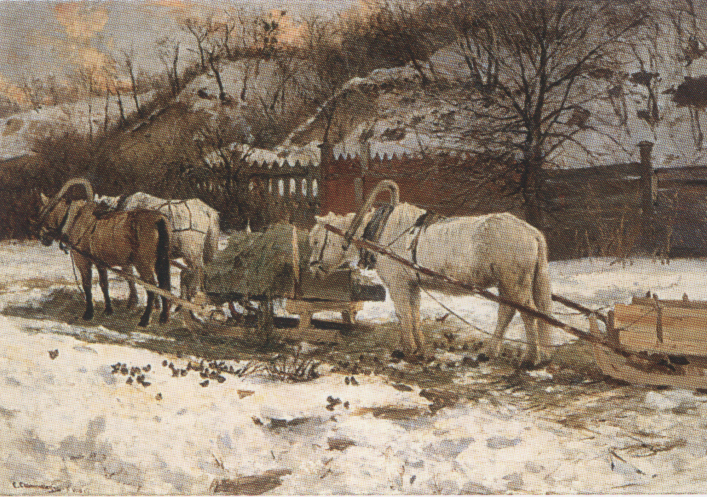
\includegraphics[width=\linewidth]{chast-kirvys/svetosl/sveto-zima.jpg}
\end{center}
\vspace*{\fill}
\newpage

А вот картина начала 20 века, «Дом художника». Наверное таким знали гости Светославского, тот же Васнецов. Глядя на полотно кажется, что пахнет цветами.

\begin{center}
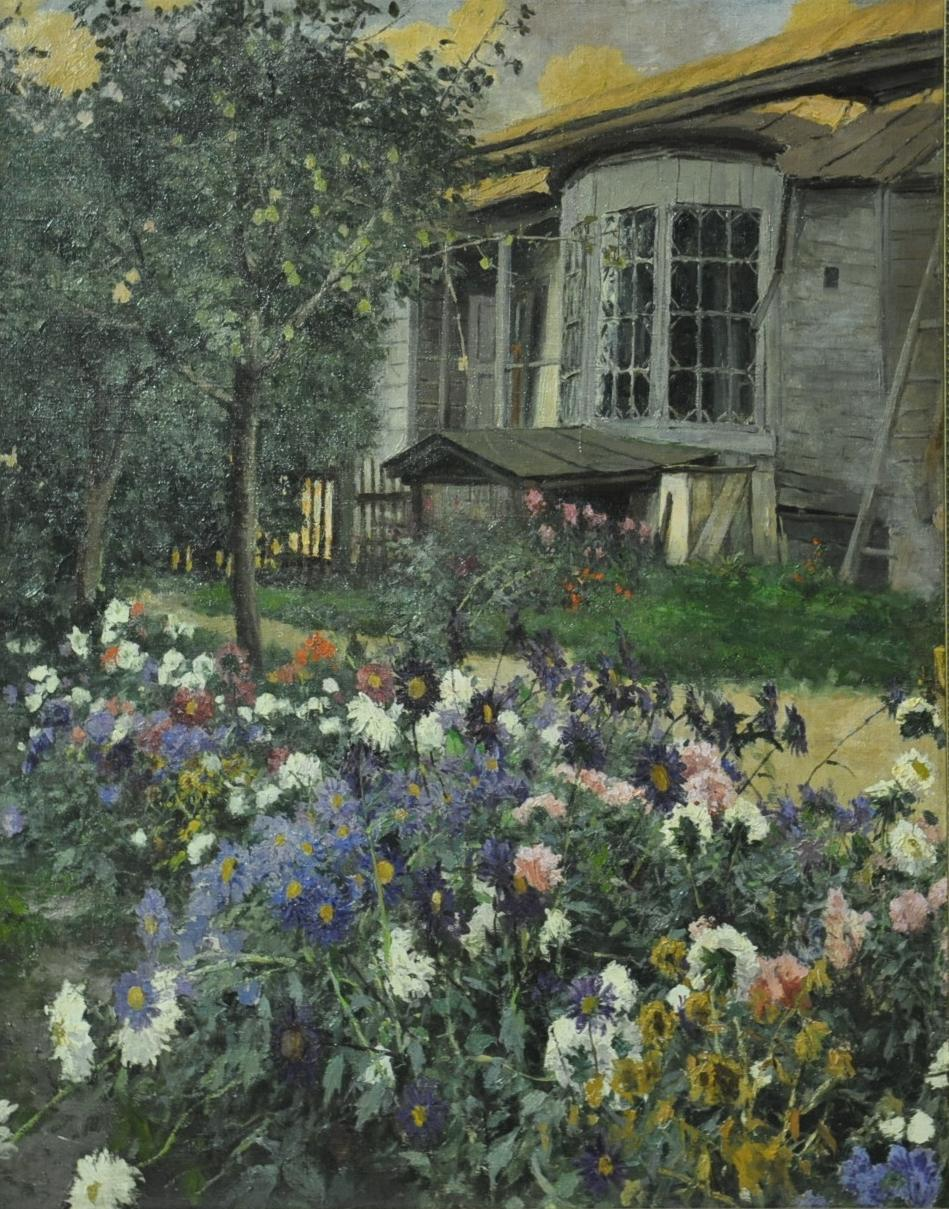
\includegraphics[width=\linewidth]{chast-kirvys/svetosl/sveto-dom-hud-good.jpg}
\end{center}

И далее работа «Осень. К концу дня». Я не пойму ракурс. Предложу две трактовки. Первая, упрощенная – что мы находимся лицом к Кирилловским высотам, и тогда за спиной у нас будет Кирилловская улица. Другая – на заднем плане отрог горы, а мы стоим на гати или мосту через овраг, и за нашей спиной – второй берег оврага (другой отрог), и Кирилловская улица будет по левую руку. Последнее кажется мне вероятнее.

\begin{center}
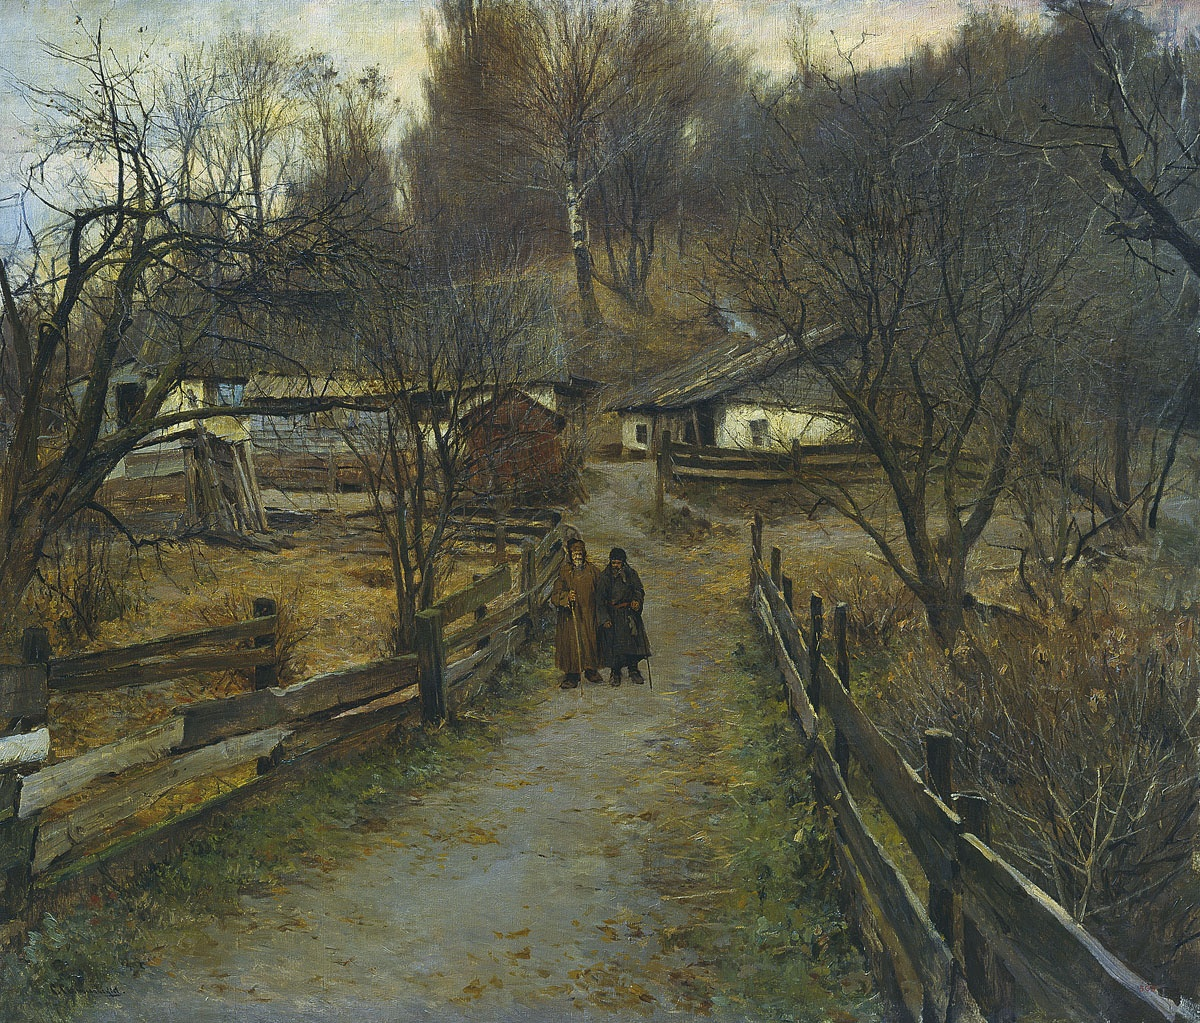
\includegraphics[width=\linewidth]{chast-kirvys/svetosl/sveto-osen-k-koncu-dnya.jpg}
\end{center}

Последний аккорд. Над местом, где была усадьба художника, нынче проложен переулок Шишкинский.

В начале 21 века здесь умирали старые дома, а их развалины догнивали под дождями и зарастали бурьяном. Я сфотографировал Шишкинский в 2005-м, а спустя десять лет по левую сторону начали возводить жилой комплекс Нагорный. Переулок, плотно застроенный коттеджами и многоэтажками, сейчас уже ничем не отличается от обычного, переделанного под богатые терема, новокиевского частного сектора. Хотя и в 2014 году сохранилась пара пустырей – прежних частных усадеб – и два-три старых домика. Двухтрубный под номером 10 вы увидите на третьем снимке. Он как стоял облупленный, с дранкой наружу, так и стоит.

\newpage
\vspace*{\fill}
\begin{center}
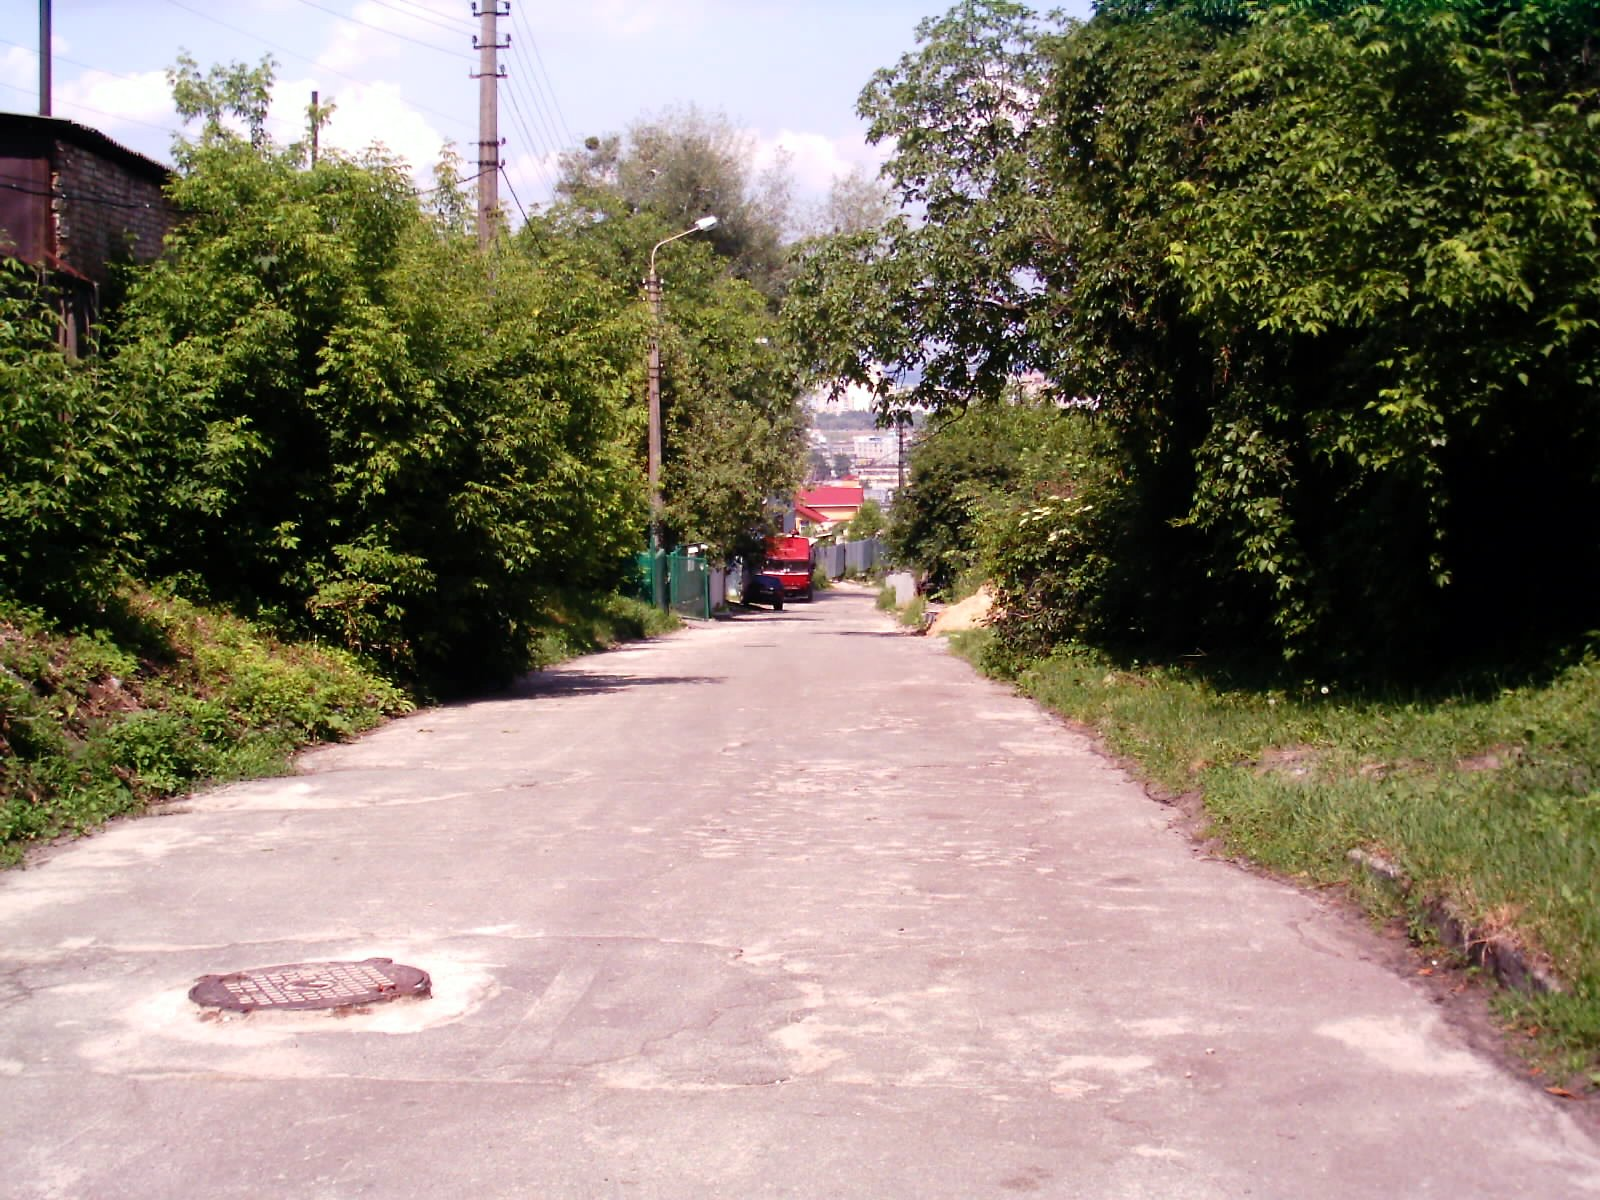
\includegraphics[width=\linewidth]{chast-kirvys/svetosl/shishk-imag0018.jpg}
\end{center}

\begin{center}
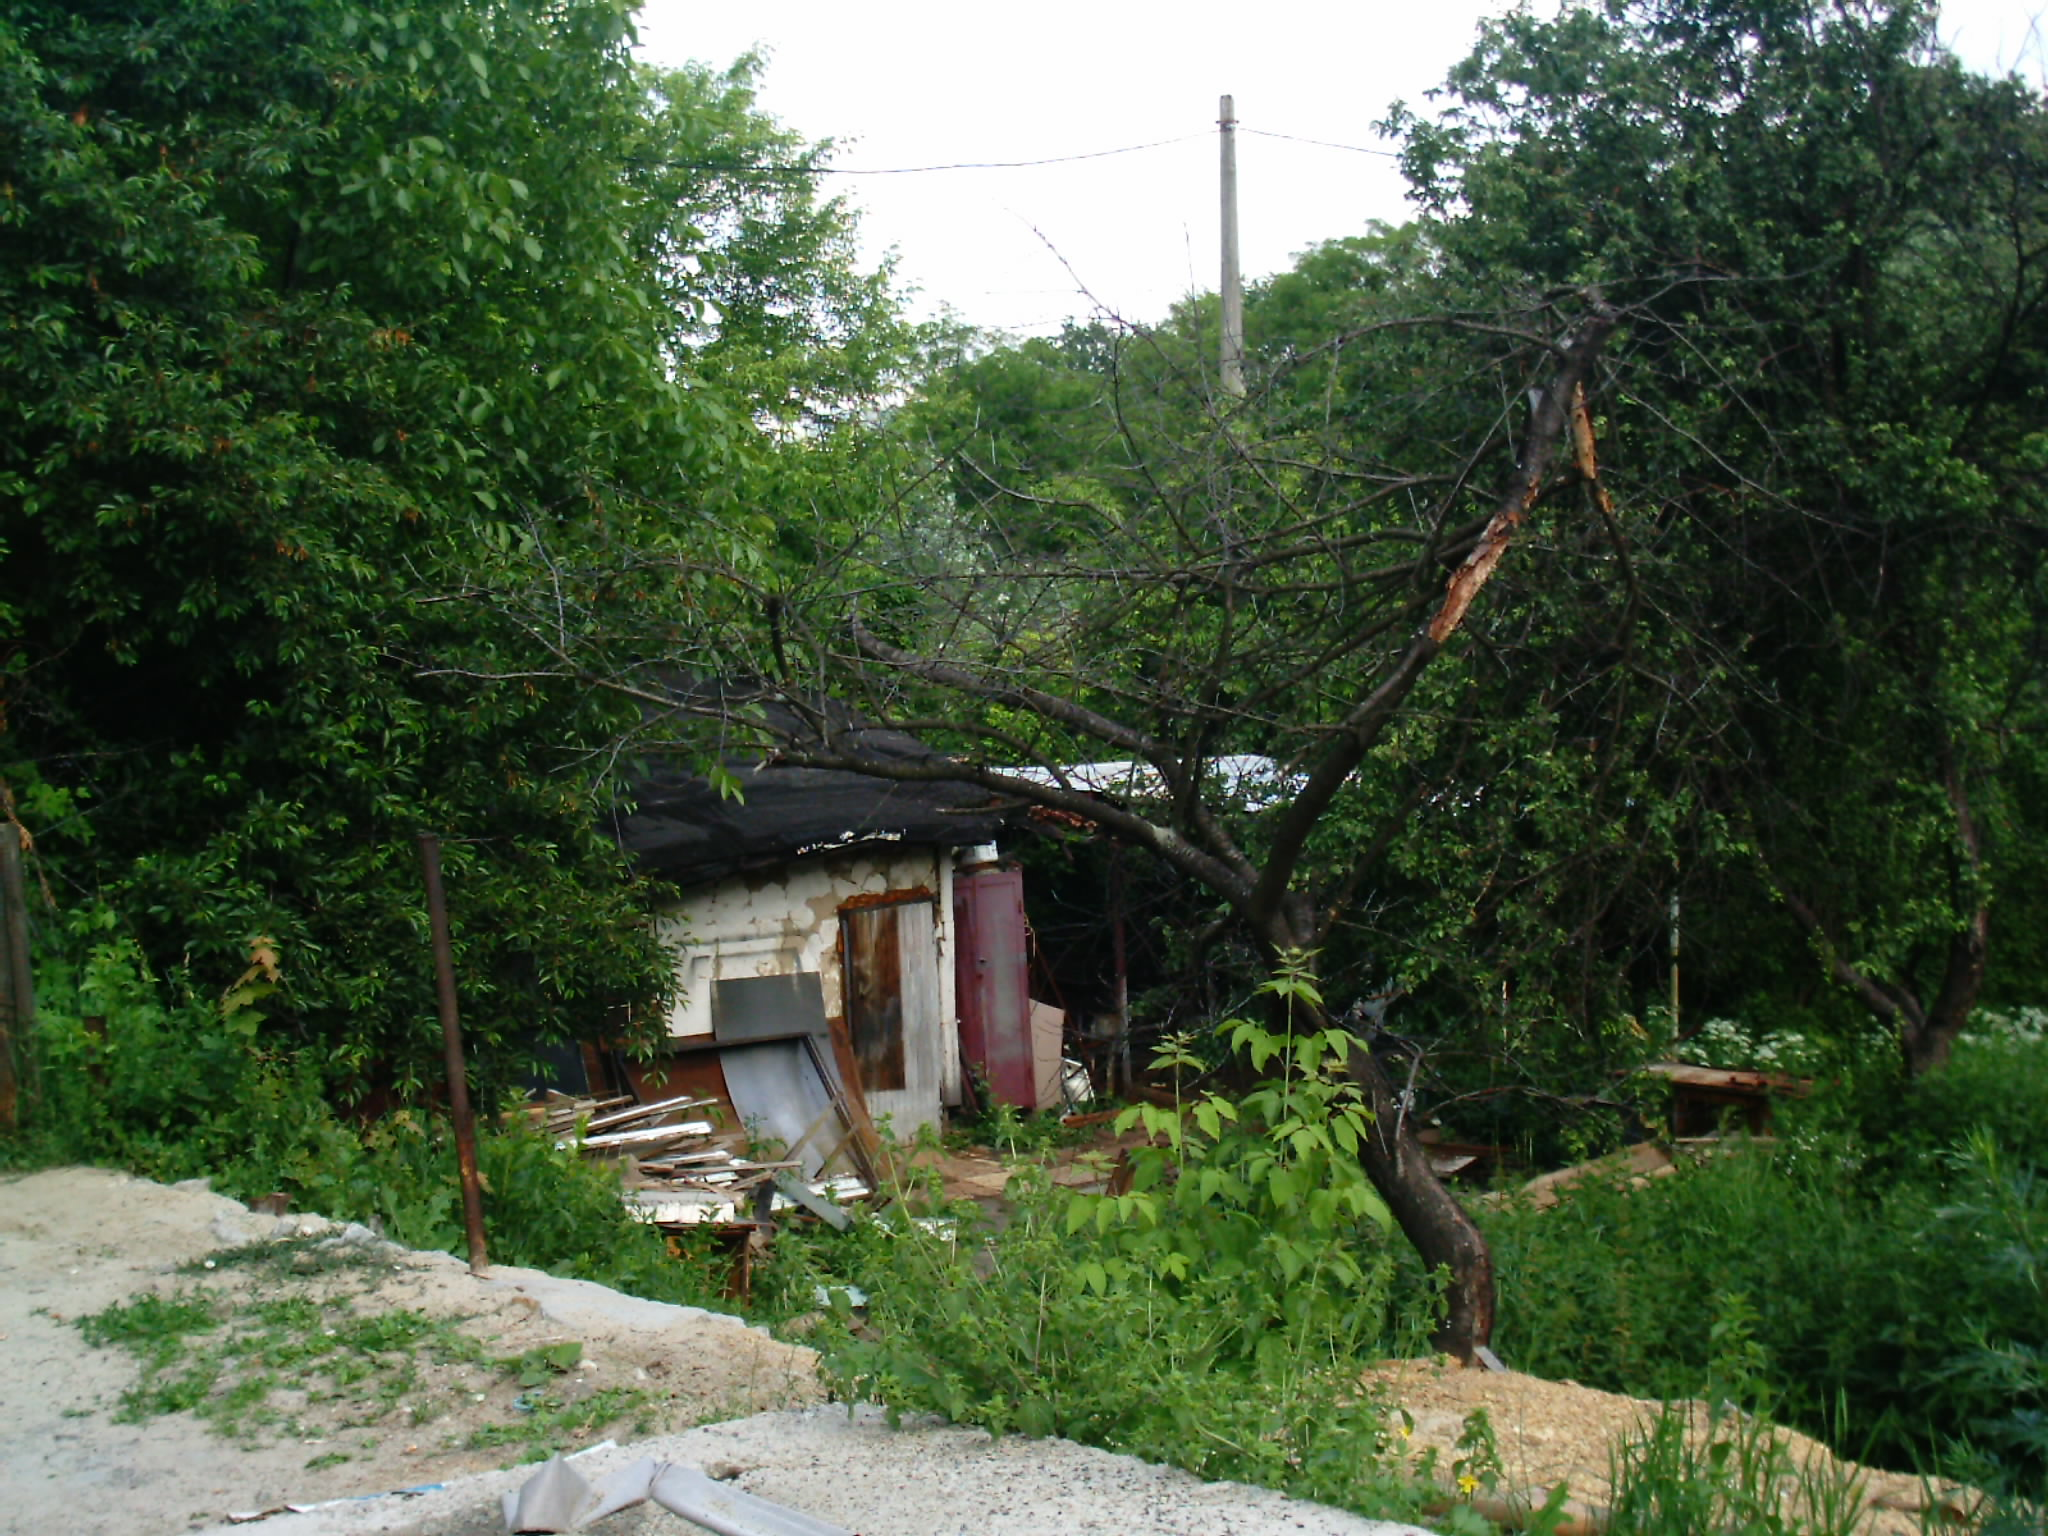
\includegraphics[width=\linewidth]{chast-kirvys/svetosl/shishk-imag0030.jpg}
\end{center}
\vspace*{\fill}

\newpage
\vspace*{\fill}
\begin{center}
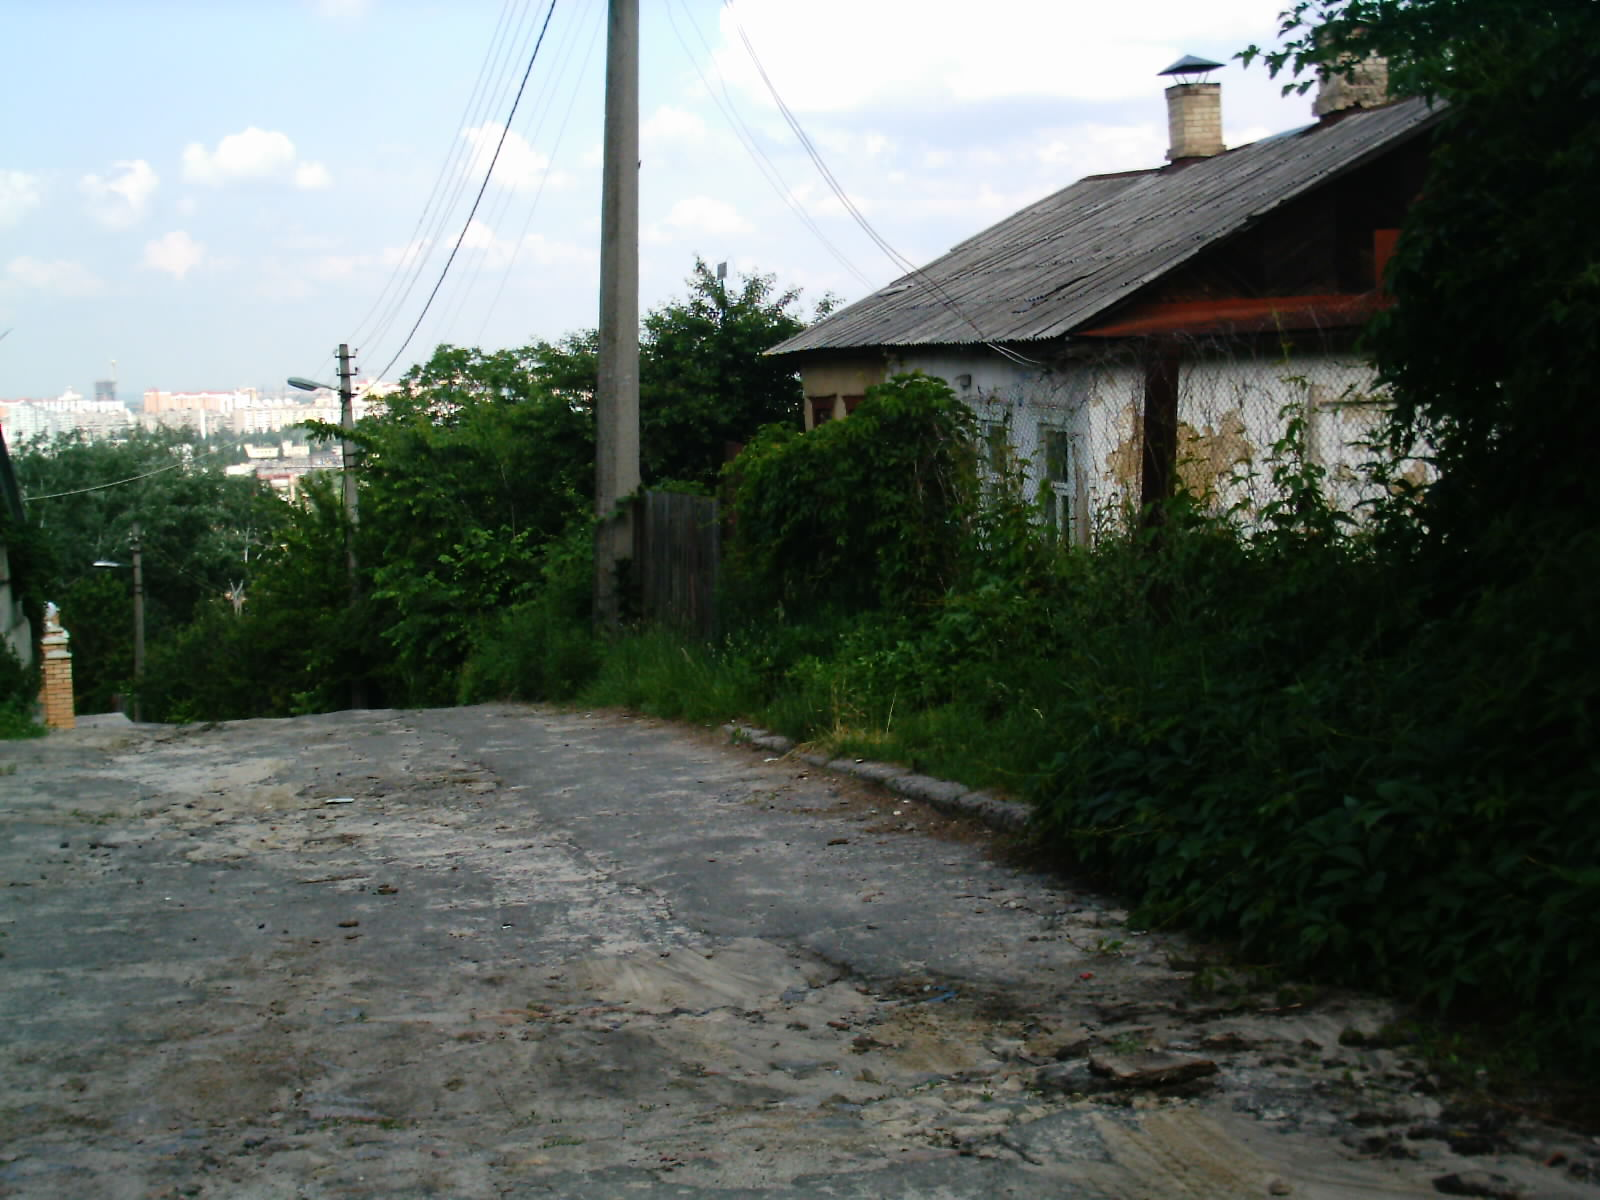
\includegraphics[width=\linewidth]{chast-kirvys/svetosl/shishk-imag0035.jpg}
\end{center}

\begin{center}
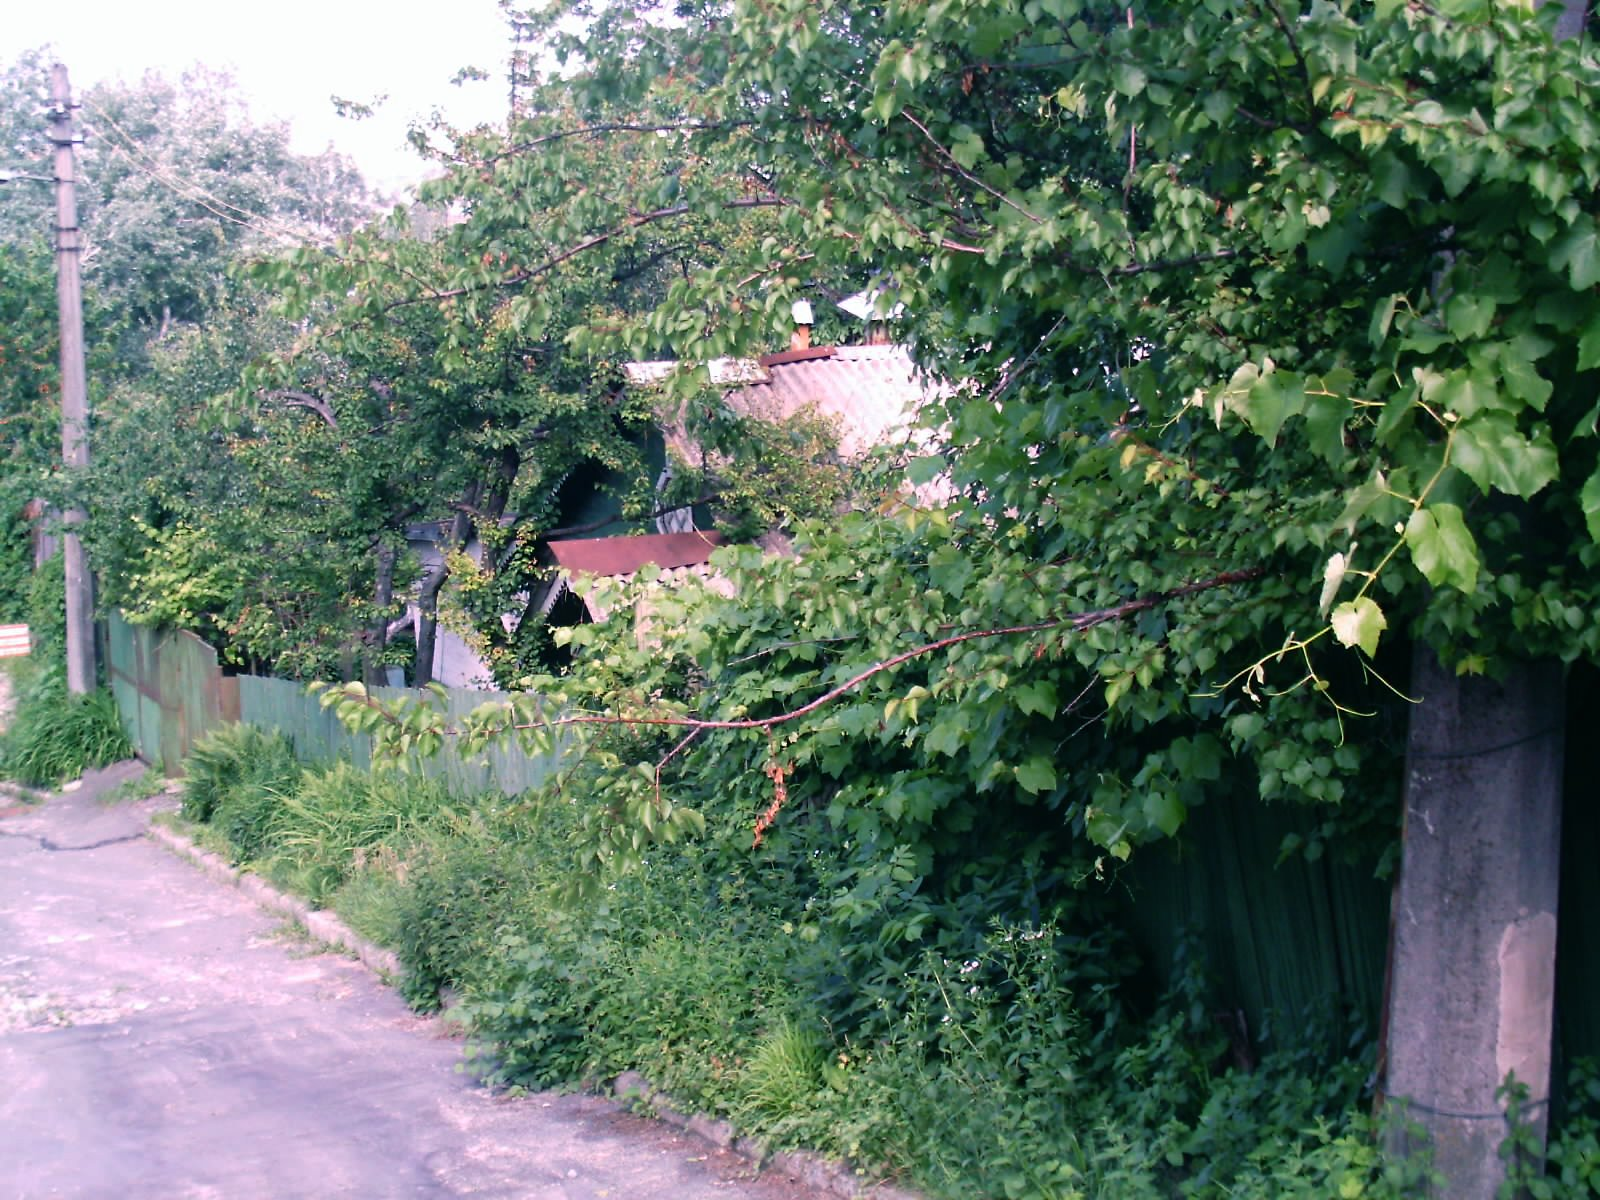
\includegraphics[width=\linewidth]{chast-kirvys/svetosl/shishk-imag0041.jpg}
\end{center}

\vspace*{\fill}
\newpage

К чему я заговорил о Шишкинском переулке? 

%А если бы те, кто дают имена улицам, знали и других художников, кроме Шишкина, творчество которого я очень уважаю, то не отнимали бы у переулка прежнее название. А может, дело сложнее.

Как известно по воспоминаниям сына Васнецова, он ходил с отцом в гости на «гору Светославского». Так слыла местность сия.

На стыке 19 и 20 веков, здесь возник Святославский переулок\footnote{На одной из карт – улица Святослава.}. Разница в одну букву незначительна, а по справочникам тех лет видно, что фамилию художника и его брата писали то через «е», то через «я». Переулок нарекли именно по близлежащей усадьбе Светославских. 

Не зная этого, в справочниках нынче привязывают князя Святослава, ну да справочникам простительно. А вот кто в 1939 году вздумал память одного художника вытеснить памятью другого, неведомо. Этот неизвестный и дал переулку новое имя – Шишкинский. Хорошо хоть не в свою честь!

Я поначалу думал – это по незнанию переименовали. Но слишком уж явным кажется замена фамилий Светославского – большого художника-пейзажиста на Шишкина, большого художника-пейзажиста! В том же 39-м близлежащие улицы тоже переименовали – появился переулок Репина, и улица Тропинина. Но Репин и Тропинин – не пейзажисты! 

Значит, возможен злой умысел – кто-то разбирался хотя бы в жанрах живописи и нарочно вытравил фамилию Светославского.

В этих же краях жил, переехав с Гоголевской, и другой известный пейзажист, Николай Корнилович Пимоненко – по адресу Верхне-Юрковская, 12\footnote{Пимоненко умер 26 марта 1912 года (нигде не могу разыскать причину смерти), до начала судебного процесса над Бейлисом, где не принимал участия, однако в деле мельком упоминается его сестра.}.

Пимоненко и Светославский пересекались не только как художники-передвижники. Оба в свое время сватались к Саше Орловской, дочери профессора живописи Владимира Орловского. Светославский и Пимоненко были у него в Питере учениками. И вот Орловский поселился в Киеве. Пимоненко со Светославским стали ходить к нему в гости, подружились, пользовались его библиотекой и оба влюбились в Сашу. Светославский признался ей в любви, но Саша ответила, что ее сердце уже занято – Николаем Пимоненко. Николай женился на ней и они вместе прожили 20 лет в усадьбе того же Орловского, на улице Гоголевской. 

%Картины самого Орловского мы уже обсуждали в главе о Почайне, на их примере хорошо видно устье этой реки до его расширения Гаванью. Добротные полотна Орловского можно рассматривать часами, подпитываясь впечатлениями.

В 2020 году по улице Кирилловской, вдоль склонов, начиная от Смородинского спуска и до пересечения Кирилловской с улицей Нахимова, нет никаких зданий, кроме трансформаторной подстанции РП-13 (Кирилловская, 83), и хозяйственного с виду строения, за бетонной оградой, под нумером 73-А. За ним начинается полукруглый овраг между мысом Смородинского спуска и другим отрогом, что граничит с яром в усадьбе Светославского. Дно оврага укреплено и приводит к забору частного дома.

На приведенном в этой главе аэрофотоснимке этот овраг находится в левой части красного квадрата, образуя, при виде сверху, как бы половину круга или монеты.

По сведениям \cite{ivancov} археолога Ивана Иванцова (1904\--1941), в 1937 году, по адресу Кирилловская, 75 (полагаю, на отрезке от нынешних 73-А и 83, промеж Смородинским спуском и упомянутым оврагом) у подножия холма раскопали\footnote{Работы велись от Киевского Центрального Исторического музея.} площадку 5х5,5 метров со следами массового трупосожжения. Слой останков составил около метра – по прикидкам ученых, тут спалили несколько сотен людей. Нижние слои, в отличие от верхних, не перегорели полностью. Некоторые скелеты лежали группами. Среди костей нашли обломки стеклянных браслетов, каменные крестики, бусины, посуду. По предметам археологи установили датировку 11-13 веков, но верно ли? Во всяком случае, дело очень давнее.

Что послужило причиной стольких смертей? Почему тела сжигались, и почему именно здесь? Как это – сжечь на небольшой площадке сотни людей? Все сразу они бы не поместились на 27,5 квадратных метрах. Значит, трупы сжигались не одновременно. Быть может эти сожжения происходили на большом отрезке времени. Христиане (а на принадлежность к этой вере будто указывают крестики, стало быть по крайней мере часть покойных была христианами) хоронили своих, закапывая в землю. Погибшие от мора не были исключениями – вспомним, почему стала кладбищем Щекавица. Да и не все погане совершали трупосожжение умерших, тоже хоронили в гробах.

А тут – площадка, где преданы огню сотни тел.

Светославский жил совсем рядом, а Хвойка – всего в двух сотнях метров. Между домом Хвойки и усадьбой Светославского – начало дороги, ведущей к логову Змиеву. Смородинский спуск.
